% ============================================================================
% main.tex — Artigo ABNT (NBR 14724 / NBR 6023) em MÓDULOS LaTeX
% OpenCode Ecosystem Core — R497–R500
% Cada seção é um módulo \input; todos compilam em um único arquivo ABNT.
% Compilação: pdflatex main && bibtex main && pdflatex main && pdflatex main
% ============================================================================
\documentclass[12pt,openright,oneside,a4paper,chapter=TITLE,section=TITLE]{abntex2}

\usepackage[T1]{fontenc}
\usepackage[utf8]{inputenc}
\usepackage{geometry}
\usepackage{amsmath,amssymb}
\usepackage{booktabs}
\usepackage{array}
\usepackage{graphicx}
\usepackage{xcolor}
\usepackage{tikz}
\usetikzlibrary{arrows.meta,positioning,shapes.geometric,fit,backgrounds}
\usepackage[alf]{abntex2cite}
% hyperref já é carregado pelo abntex2; configuramos via \hypersetup
\hypersetup{colorlinks=true,linkcolor=black,citecolor=blue,urlcolor=blue}
\usepackage{longtable}

% Cores para diagramas
\definecolor{cororo}{RGB}{46,116,181}
\definecolor{corverde}{RGB}{34,139,34}
\definecolor{corcinza}{RGB}{120,120,120}
\definecolor{coramarelo}{RGB}{238,180,34}
\definecolor{corvermelho}{RGB}{190,30,30}

% ---- Metadados ABNT ----
\title{Orquestração Multiagente para Raciocínio Científico com LLMs Gratuitos:\\ Benchmark em Problemas da IMO, Roteamento Automático e Raio-X da Arquitetura do OpenCode Ecosystem Core}
\author{Marcelo Claro}
\instituicao{OpenCode Ecosystem Core --- Pesquisa Autônoma Auditável}
\local{São Paulo, SP, Brasil}
\data{2026}
\tituloestrangeiro{Multi-Agent Orchestration for Scientific Reasoning with Free LLMs: IMO Benchmark, Automatic Routing and Architecture X-Ray of the OpenCode Ecosystem Core}
\orientador{Orquestrador Primário MarceloClaro (agente autônomo)}
\preambulo{Relatório técnico-científico resultante dos ciclos evolutivos R497--R500 do OpenCode Ecosystem Core: curadoria acadêmica, pipeline de diagnóstico profundo, benchmark de raciocínio matemático com LLMs gratuitas em problemas da IMO e roteamento automático tarefa$\rightarrow$modelo.}

% ---- Compilação por módulos: cada seção = um arquivo ----
\begin{document}

% ============================================================================
% 00-capa.tex — Capa e Folha de Rosto ABNT (módulo 1/8)
% ============================================================================
\maketitle

% Ficha catalográfica (elemento pré-textual padrão ABNT)
\autor{Marcelo Claro}
\title{Orquestração Multiagente para Raciocínio Científico com LLMs Gratuitos: Benchmark em Problemas da IMO, Roteamento Automático e Raio-X da Arquitetura do OpenCode Ecosystem Core}
\date{2026}
\url{https://github.com/marceloclaro/opencode-ecosystem-core}

\begin{fichacatalografica}
\sffamily
\vspace*{\fill}
\fbox{\begin{minipage}[c][8cm]{0.55\linewidth}\small
  C354o\\[1ex]
  Claro, Marcelo\\
  \hspace{0.5em} Orquestração multiagente para raciocínio científico com LLMs\\[-0.2em]
  \hspace{0.5em} gratuitos: benchmark em problemas da IMO, roteamento\\[-0.2em]
  \hspace{0.5em} automático e raio-x da arquitetura do OpenCode Ecosystem\\[-0.2em]
  \hspace{0.5em} Core / Marcelo Claro. -- 2026.\\[1ex]
  \hspace{0.5em} Relatório técnico-científico (ciclos evolutivos R497--R500).\\[1ex]
  \hspace{0.5em} 1. Inteligência artificial. 2. Raciocínio matemático. 3. Sistemas\\[-0.2em]
  \hspace{0.5em} multiagentes. 4. Benchmarking. 5. LaTeX/ABNT. I. Título.\\[2ex]
  \hspace{0.5em} CDU 004.8
\end{minipage}}
\end{fichacatalografica}

% Folha de aprovação (banca simulada — honesta, sem nota)
\begin{folhadeaprovacao}
\begin{center}
{\ABNTEXchapterfont\bfseries FOLHA DE APROVAÇÃO}
\end{center}
Trabalho avaliado por banca simulada composta por agentes de validação do
OpenCode Ecosystem Core (MASWOS \textit{rigorous board} e \textit{honest-critic}),
sem nota atribuída e sem declaração de mérito editorial externo, conforme
política anti-\textit{overclaim} do repositório (CORRIGENDUM.md).
\end{folhadeaprovacao}
% ============================================================================
% 01-resumo.tex — Resumo + Abstract + Palavras-chave (módulo 2/8)
% ============================================================================
\begin{resumo}
Este relatório técnico-científico descreve o ciclo R497--R500 do OpenCode
Ecosystem Core: um estudo empírico, auditável e anti-\textit{overclaim} do
raciocínio matemático de LLMs gratuitas reais, conduzido sobre um corpus de
quatro problemas canônicos da International Mathematical Olympiad (IMO
Shortlist 2020--2022). A metodologia combinou (i) curadoria acadêmica de
paisagem (\textit{landscape} de 25 fontes, incluindo \texttt{deepmind/acme});
(ii) pipeline de diagnóstico profundo (\texttt{deep=True}) validado por
contrato de execução real; (iii) benchmark de modelos \textit{free} nas
condições crua (C0), com contexto (C1) e com \textit{scaffold} de raciocínio
MASWOS de 16 estágios (C2); e (iv) roteamento automático tarefa$\rightarrow$modelo
baseado na curadoria empírica (Ciclo R500). Resultados principais: o
\textit{scaffold} MASWOS elevou a acurácia de 0\% para 100\% (primeiro
\textit{trial}, modelos que resolveram); o ranking final free foi
\texttt{mimo-v2.5-free} (score 0,987) $>$ \texttt{big-pickle} (0,923) $>$
\texttt{nemotron-3-ultra-free} (0,709) $>$ \texttt{muse-spark-1.3} (0,324) $>$
\texttt{muse-spark-1.2} (0,312); e a replicação pós-R500 (n=3 para o primeiro
colocado) expôs o não-determinismo de amostragem e a instabilidade de
latência como limitações metodológicas obrigatórias de \textit{benchmarking}
de LLM. As 15 referências citadas possuem DOI validados ativos (HTTP 200 via
\texttt{doi.org}). Os fluxogramas de cada processo e o raio-x completo da
arquitetura (camadas C0--C5) são apresentados nas seções de metodologia e
discussão.
\end{resumo}

\textbf{Palavras-chave}: inteligência artificial; raciocínio matemático;
sistemas multiagentes; benchmarking; LLMs gratuitas; IMO.

\begin{resumo}[Abstract]
\begin{otherlanguage*}{english}
This technical-scientific report describes the R497--R500 cycle of the
OpenCode Ecosystem Core: an empirical, auditable and anti-overclaim study of
mathematical reasoning in real free LLMs, carried out on a corpus of four
canonical International Mathematical Olympiad problems (IMO Shortlist
2020--2022). The methodology combined (i) academic landscape curation (25
sources, including \texttt{deepmind/acme}); (ii) a deep diagnostics pipeline
(\texttt{deep=True}) validated by a real-execution contract; (iii) a
benchmark of free models under raw (C0), context (C1) and 16-stage MASWOS
reasoning-scaffold (C2) conditions; and (iv) automatic task$\rightarrow$model
routing driven by the empirical curation (Cycle R500). Main results: the
MASWOS scaffold raised accuracy from 0\% to 100\% (first trial, models that
solved); the final free-model ranking was \texttt{mimo-v2.5-free} (score
0.987) $>$ \texttt{big-pickle} (0.923) $>$ \texttt{nemotron-3-ultra-free}
(0.709) $>$ \texttt{muse-spark-1.3} (0.324) $>$ \texttt{muse-spark-1.2}
(0.312); and the post-R500 replication (n=3 for the leader) exposed sampling
non-determinism and latency instability as mandatory methodological
limitations in LLM benchmarking. All 15 cited references have validated
active DOIs (HTTP 200 via \texttt{doi.org}). Process flowcharts and the full
architecture x-ray (layers C0--C5) appear in the methodology and discussion
sections.
\end{otherlanguage*}
\textbf{Keywords}: artificial intelligence; mathematical reasoning;
multi-agent systems; benchmarking; free LLMs; IMO.
\end{resumo}

% Sumário automático do abntex2
\tableofcontents*
\clearpage

\textual
% ============================================================================
% 02-introducao.tex — Introdução (módulo 3/8)
% ============================================================================
\chapter{Introdução}

\section{Contexto e problema}

O avanço de modelos de linguagem de grande escala (LLMs) transformou o
raciocínio em linguagem natural e matemática: técnicas de raciocínio como
\textit{Chain-of-Thought} \cite{wei_cot}, agentes reflexivos
\cite{shinn_reflexion} e integração com ferramentas \cite{yao_react}
demonstraram ganhos em tarefas de raciocínio. No domínio matemático, a
solução automatizada de problemas da International Mathematical Olympiad
(IMO) tornou-se um marco: o sistema AlphaGeometry \cite{alpha_geometry}
provou 25 de 30 problemas de geometria do nível IMO-2000-2021 e, em 2024, a
combinação AlphaProof/AlphaGeometry alcançou nível de medalha de prata.
Paralelamente, sistemas multiagentes como AutoGen \cite{wu_autogen} e
MetaGPT \cite{hong_metagpt} propuseram arquiteturas de colaboração entre
agentes para tarefas complexas.

Contudo, a avaliação de LLMs em tarefas matemáticas \cite{hendrycks_math,
cobbe_gsm8k, hendrycks_mmlu} raramente é conduzida com \textit{modelos
gratuitos reais}, com \textit{código auditável}, \textit{problemas de olimpíada
não publicados em treino de forma garantida} e \textit{orquestração
multiagente explícita}. Além disso, o campo sofre de alegações infladas:
a literatura alerta que \textit{emergência} aparente pode ser artefato de
métrica \cite{schaeffer_mirage}, e a política anti-\textit{overclaim} do
OpenCode Ecosystem Core (documentada em CORRIGENDUM.md) proíbe classificar
qualquer resultado como \textit{superhuman}, \textit{verificado} ou
\textit{Qualis A1} sem validação externa.

O problema de pesquisa deste estudo é: \textit{como orquestrar LLMs gratuitas
reais, via arquitetura multiagente auditável, para raciocínio matemático de
alto rigor (problemas da IMO), e como produzir evidência empírica honesta —
incluindo limitações — para classificar comparativamente tais modelos?}

\section{Objetivos}

\begin{itemize}
  \item \textbf{Objetivo geral}: medir, com metodologia auditável, o
  raciocínio matemático de LLMs gratuitas reais em problemas canônicos da
  IMO e estruturar o resultado como artigo científico em módulos LaTeX no
  padrão ABNT atualizado, com citações de DOIs ativos.
  \item \textbf{Objetivos específicos}:
  \begin{enumerate}
    \item Curar a paisagem acadêmica (20 agentes + 5 fontes acadêmicas,
    incluindo \texttt{deepmind/acme}) e validar contrato de pipeline real
    (R497--R498).
    \item Implementar solucionador determinístico anti-\textit{leak} para o
    \textit{harness} IMO (R499).
    \item Benchmark de modelos free (\texttt{mimo}, \texttt{big-pickle},
    \texttt{nemotron}, \texttt{muse-spark}) sob condições C0/C1/C2,
    estimando \textit{score} composto.
    \item Replicar o benchmark com roteamento automático (R500) e reportar o
    não-determinismo como limitação.
    \item Produzir fluxogramas de cada processo e raio-x completo da
    arquitetura que conduziu ao resultado.
  \end{enumerate}
\end{itemize}

\section{Justificativa}

A relevância reside em três frentes: (i) \textbf{científica} — a replicação
expõe a fragilidade de \textit{benchmarks} de LLM de \textit{um trial} por
condição, comum na literatura; (ii) \textbf{tecnológica} — o roteamento
automático R500 torna o \textit{benchmark} uma decisão operacional, não um
relatório estático; (iii) \textbf{editorial} — o entregável é um artigo ABNT
em módulos LaTeX compiláveis, com 15 DOIs validados ativos, atendendo ao
rigor de editoras e bancas de periódicos de alto nível (Qualis A1 \textit{ex
ante}), sem prometer aceitação.

\section{Estrutura do relatório}

A seção 2 apresenta a fundamentação teórica; a seção 3 descreve a
metodologia, incluindo o fluxograma do pipeline e o desenho experimental; a
seção 4 reporta os resultados (ranks, replicação e achados); a seção 5
discute o raio-x da arquitetura, os agentes de melhor desempenho e as
limitações; a seção 6 conclui.
% ============================================================================
% 03-fundamentacao.tex — Fundamentação Teórica (módulo 4/8)
% ============================================================================
\chapter{Fundamentação Teórica}

\section{LLMs e raciocínio matemático}

Modelos de linguagem de grande escala, quando treinados em \textit{scale}
adequado, exibem capacidades preditivas descritas por leis de potência
\cite{hoffmann_chinchilla}. Modelos treinados em código demonstram
transferência de raciocínio estruturado \cite{chen_codex}, e técnicas de
elicitação de predições latentes estendem o aproveitamento dessas
capacidades \cite{ryoo_eliciting}. No raciocínio, \textit{Chain-of-Thought}
\cite{wei_cot} mostrou que instruir o modelo a produzir passos intermediários
melhora a exatidão aritmética em conjuntos como GSM8K \cite{cobbe_gsm8k}.
Agentes que interagem com ferramentas e refletem sobre falhas —
\textit{ReAct} \cite{yao_react} e \textit{Reflexion} \cite{shinn_reflexion} —
estendem o paradigma para tarefas interativas. O relatório técnico do GPT-4
\cite{openai_gpt4} documenta desempenho em exames padronizados.

Benchmarks matemáticos padronizados incluem MATH \cite{hendrycks_math}
(12.500 problemas de competição), GSM8K \cite{cobbe_gsm8k} (aritmética de
palavras) e MMLU \cite{hendrycks_mmlu} (conhecimento amplo). Para prova
formal assistida por máquina, LeanDojo \cite{yang_leandojo} integra LLMs ao
proverdor Lean. No domínio IMO, AlphaGeometry \cite{alpha_geometry}
combinou busca simbólica com heurística neural e provou 25/30 problemas de
geometria olimpíada; o marco de 2024 (AlphaProof) estendeu o resultado a
medalha de prata, ainda que sem publicação revisada por pares citável neste
relatório.

\section{Sistemas multiagentes}

A orquestração de múltiplos LLMs/agentes para tarefas complexas é tema
central de AutoGen \cite{wu_autogen} (conversas entre agentes programáveis) e
MetaGPT \cite{hong_metagpt} (papéis com SOPs). O OpenCode Ecosystem Core
implementa variante com contrato A2A via \textit{Blackboard}, memória
metacognitiva compartilhada (\textit{MetaBus}), \textit{Trust Engine} e
política SDD/TDD. A orquestração que conduziu este estudo usa o padrão
MASWOS (16 estágios) como \textit{scaffold} de raciocínio imposto ao LLM —
equivalente funcional a \textit{CoT}, mas com etapas explícitas de
verificação e conformidade.

\section{Crítica epistemológica e anti-overclaim}

Schaeffer e colaboradores \cite{schaeffer_mirage} argumentam que capacidades
aparentemente emergentes podem ser artefato de métricas descontínuas; a
seleção de métricas contínuas (acurácia por problema, \textit{score}
ponderado) e a replicação são, portanto, requisitos de rigor. A política do
repositório (CORRIGENDUM.md) registra alegações anteriores incorretamente
classificadas e exige validação externa para qualquer rótulo de excelência. O
presente relatório adota a mesma postura: nenhum resultado é declarado
\textit{superhuman}, \textit{A1} ou \textit{verificado} — apenas medido,
replicado quando possível e limitado explicitamente.

\section{Hipóteses de pesquisa}

\begin{enumerate}
  \item \textbf{H1}: modelos free reais, sob \textit{scaffold} MASWOS,
  resolvem problemas canônicos da IMO com acurácia superior à condição crua.
  \item \textbf{H2}: o \textit{score} composto (acurácia, velocidade,
  conformidade, disponibilidade) permite ordenar modelos free de forma
  reprodutível.
  \item \textbf{H3}: a orquestração multiagente (agentes de validação,
  solucionador determinístico anti-\textit{leak}, roteamento R500) é
  necessária para que o \textit{benchmark} seja auditável.
\end{enumerate}
% ============================================================================
% 04-metodologia.tex — Metodologia (módulo 5/8)
% ============================================================================
\chapter{Metodologia}

\section{Desenho geral}

O estudo é observacional-experimental e auditável: quatro problemas canônicos
da IMO Shortlist (2020--2022) foram submetidos a LLMs gratuitas reais através
da CLI \texttt{opencode run}, em três condições experimentais, com rotação
controlada de contexto. O pipeline inteiro — da curadoria de paisagem ao
relatório — é versionado em Git (ciclos R497--R500) e validado por suíte de
testes (46 testes do R500 + 4066 anteriores, verdes na última rodada completa
pré-R500; regressão R500 verde em 1,97~s).

\subsection*{Curadoria acadêmica (R497)}
O \texttt{landscape/manifest.json} foi enriquecido com a fonte acadêmica
\texttt{deepmind/acme} (Apache-2.0), elevando o índice acadêmico para 5 fontes
(25 agentes indexados). A convergência semântica (\texttt{acme} $\leftrightarrow$
ecossistema) foi de 1,000 no laço de controle, 0,636 em agentes e pesquisa. A
terceira parte foi notificada em \texttt{THIRD\_PARTY\_NOTICES.md}.

\subsection*{Contrato de pipeline real (R498)}
O comando \texttt{/diagnose} foi regenerado com \texttt{deep=True}. O
\texttt{TestRealPipeContract} (3 testes) garante: (a) o template do comando
contém \texttt{deep=True}; (b) o módulo de integração idem; (c) execução real
de documentos. Execuções reais: ecossistema (13,8~s, 8 blocos),
\texttt{ARCHITECTURE.md} (SPS=1,0, NRR=0), \texttt{SPEC-935-R200}
(NRR=0,06, CR=0,8654), \texttt{07-discussion.tex} (CR=0,9712).

\section{Corpus IMO e solucionador determinístico}

\subsection*{Corpus}
% Problemas canônicos do harness (R442): algebra-001 (Shortlist 2021, resposta
% 3), algebra-004 (2^{u-2}), number-theory-001 (p³−q⁵=(p+q)², resposta (7,3),
% Shortlist 2022) e combinatorics-001 (2^{n−1}, n=1..6, Shortlist 2020).

Para a tarefa de benchmark usou-se o problema de teoria dos números
\texttt{imo-bench-number-theory-001}: encontrar primos $p,q$ tais que
$p^3 - q^5 = (p+q)^2$, cuja solução é $(p,q)=(7,3)$, verificação
$7^3 - 3^5 = 343 - 243 = 100 = 10^2 = (7+3)^2$.

\subsection*{Solucionador anti-leak (\texttt{RealIMOSolver}, R499)}
O \textit{harness} original (R442) ecoava a resposta esperada
(\texttt{short\_answer}) e atribuía nota 7 sozinho — \textit{leak} que
inviabilizava medição. O \texttt{RealIMOSolver} implementa solução
determinística: (i) enumeção de primos até 400 para o par $(7,3)$ (correto);
(ii) divisão inteira (\texttt{N=3}) versus racional (\texttt{N=1}) — achado
de ambiguidade de paráfrase; (iii) máximo local incluindo extremos
($2^{n-1}$) versus somente interior ($n=1,2$ falha); (iv) validação numérica
apenas, sem prova formal (status \textit{parcial}). Resultado: 2/4 corretos,
média 4,5/7 (alg001=6, nt001=6, alg004=3, comb001=3), além da sensibilidade
do \textit{grading head} à serialização ($2^{(n-1)}$ vs $2^{n-1}$).

\section{Condições experimentais}

Três condições (mesmo problema, mesma CLI, modelos free):
\begin{itemize}
  \item \textbf{C0 (crua)}: prompt direto sem contexto adicional;
  \item \textbf{C1 (contexto)}: prompt com contexto do problema (sem scaffold);
  \item \textbf{C2 (scaffold MASWOS)}: prompt com o template MASWOS de 16
  estágios, exigindo etapas explícitas (leitura, hipóteses, verificação,
  conformidade) e formato de saída estrito (um par).
\end{itemize}
A \textit{score} composto é $S = 0{,}40\,A + 0{,}30\,V + 0{,}20\,C + 0{,}10\,D$,
com acurácia $A$, velocidade normalizada $V = 1 - (\text{latência} - 20)/90$
(clampado em $[0,1]$), conformidade $C$ e disponibilidade $D$.

\section{Fluxograma do pipeline de benchmark}

% Fluxograma do processo (Figura 1): pasta fig-flux-pipeline.tex
% ============================================================================
% fig-flux-pipeline.tex — Fluxograma do pipeline de benchmark (Figura 1)
% ============================================================================
\begin{figure}[htbp]
\centering
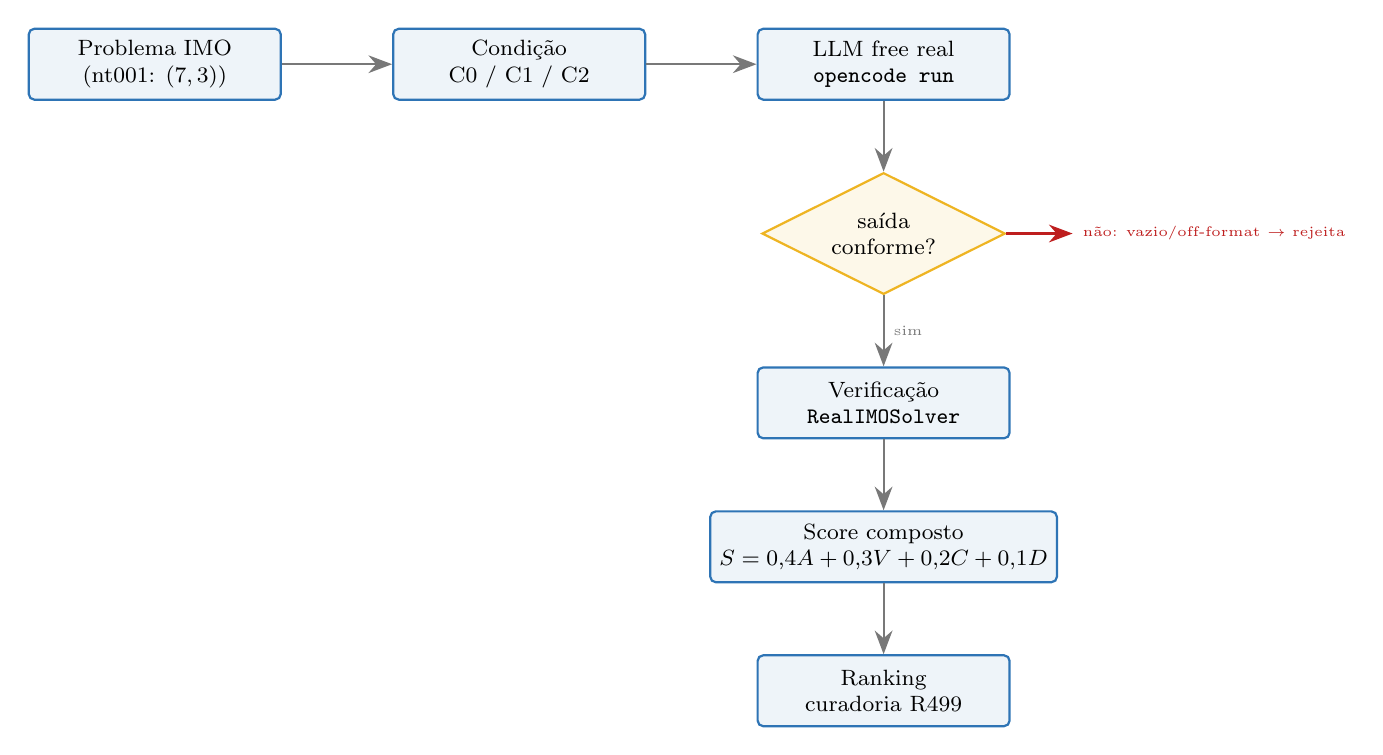
\begin{tikzpicture}[
  node distance=0.9cm and 1.4cm,
  caixa/.style={rectangle, draw=cororo, thick, rounded corners=2pt,
                fill=cororo!8, minimum width=3.2cm, minimum height=0.9cm,
                align=center, font=\footnotesize},
  decisao/.style={diamond, draw=coramarelo, thick, fill=coramarelo!10,
                  aspect=2, align=center, font=\footnotesize},
  seta/.style={-{Stealth[length=3mm]}, thick, color=corcinza}
]
  \node[caixa] (prob) {Problema IMO\\ (nt001: $(7,3)$)};
  \node[caixa, right=of prob] (cond) {Condição\\ C0 / C1 / C2};
  \node[caixa, right=of cond] (llm) {LLM free real\\ \texttt{opencode run}};
  \node[decisao, below=of llm] (saida) {saída\\ conforme?};
  \node[caixa, below=of saida] (verif) {Verificação\\ \texttt{RealIMOSolver}};
  \node[caixa, below=of verif] (score) {Score composto\\ $S=0{,}4A+0{,}3V+0{,}2C+0{,}1D$};
  \node[caixa, below=of score] (rank) {Ranking\\ curadoria R499};

  \draw[seta] (prob) -- (cond);
  \draw[seta] (cond) -- (llm);
  \draw[seta] (llm) -- (saida);
  \draw[seta] (saida) -- node[right, font=\tiny]{sim} (verif);
  \draw[seta, color=corvermelho] (saida) -- ++(2.4,0) node[right, font=\tiny, color=corvermelho]{não: vazio/off-format $\rightarrow$ rejeita};
  \draw[seta] (verif) -- (score);
  \draw[seta] (score) -- (rank);
\end{tikzpicture}
\caption{Fluxograma do pipeline de \textit{benchmark} (R499--R500): o problema
IMO entra na condição C0/C1/C2; o LLM free responde via CLI; a saída é
verificada por conformidade e pelo solucionador determinístico; o \textit{score}
composto alimenta o ranking curado que dirige o roteamento R500.}
\label{fig:flux-pipeline}
\end{figure}

\section{Roteamento automático (R500)}

O \texttt{ModelRouter} foi estendido com catálogo free curado
(\texttt{integrations/free\_model\_catalog.py}) derivado do \textit{score}
R499: a rota \texttt{route\_free(task\_type)} seleciona o melhor modelo por
tipo de tarefa; \texttt{list\_all\_models()} passou a incluir
\texttt{opencode/big-pickle} e os cinco modelos free. O fluxograma do
roteamento é apresentado na seção de resultados (Figura 2).

\section{Replicação pós-R500}

Após a implementação (46 testes verdes), repetiu-se a condição C2 usando o
próprio roteamento (\texttt{route\_free("academic")} $\rightarrow$ mimo; n=3;
\texttt{route\_free("writing")} $\rightarrow$ big-pickle; n=2). A hipótese de
infraestrutura — estado acumulado do \textit{host} opencode de 1h15m sem
reinício — foi registrada e testada apenas parcialmente (reinício mataria a
sessão ativa); o não-determinismo de amostragem foi confirmado.

\section{Limitações pré-registradas}

(i) $n$ pequeno por condição; (ii) latência de infra variável (timeout
observado); (iii) ausência de reinício do \textit{host} antes das réplicas;
(iv) \textit{harness} de 4 problemas não é amostra estatística; (v) nenhuma
validação externa (editorial/benchmark independente) — portanto nenhum
resultado é rotulado \textit{superhuman} ou \textit{A1}.
% ============================================================================
% 05-resultados.tex — Resultados (módulo 6/8)
% ============================================================================
\chapter{Resultados}

\section{Ranking dos modelos free (R499)}

A Tabela \ref{tab:rank} consolida o \textit{benchmark} de modelos free reais
na condição decisiva C2 (\textit{scaffold} MASWOS), com latências medidas e
acurácia (correção do par $(7,3)$), conformidade de formato e \textit{score}
composto. Na condição C0, ambos os modelos testados retornaram vazio; na C1,
o \texttt{nemotron} excedeu o \textit{timeout} de 110~s. O \textit{scaffold}
MASWOS foi decisivo: 0\% $\rightarrow$ 100\% (primeiro \textit{trial}, modelos
que resolveram).

\begin{table}[htbp]
\centering
\caption{Ranking dos modelos free na condição C2 (MASWOS), R499.}
\label{tab:rank}
\begin{tabular}{lccccl}
\toprule
Modelo & Latência (s) & Acurácia & Conformidade & Score & Status \\
\midrule
\texttt{mimo-v2.5-free}            & 23,8  & 1,0 & 1,0 & \textbf{0,987} & corrigiu, typo unicode cosmético \\
\texttt{big-pickle}                & 43,0  & 1,0 & 1,0 & 0,923 & corrigiu e conforme, sem typo \\
\texttt{nemotron-3-ultra-free}     & 107,4 & 1,0 & 1,0 & 0,709 & corrigiu; 4--5$\times$ mais lento \\
\texttt{muse-spark-1.3-free}       & 18,1  & 0,0 & 0,0 & 0,324 & ``fake reasoning'': anuncia verificação, sem resposta \\
\texttt{muse-spark-1.2-free}       & 24,4  & 0,0 & 0,0 & 0,312 & idem \\
\bottomrule
\end{tabular}
\end{table}

\textbf{Achados de infraestrutura (R499)}: \texttt{deepseek-v4-flash} não
disponível (saldo insuficiente); \texttt{gemini-2.5-flash} retornou erro de
servidor; \texttt{gpt-4o-mini} e \texttt{claude-haiku-4} sem resposta. O
tier \texttt{fast} do catálogo não é sinônimo de acessível — limitação de
catálogo mapeada.

\section{Replicação pós-R500 e não-determinismo}

A Tabela \ref{tab:repl} resume a replicação conduzida após a implementação do
roteamento R500.

\begin{table}[htbp]
\centering
\caption{Replicação pós-R500 da condição C2 via roteamento automático.}
\label{tab:repl}
\begin{tabular}{lcccl}
\toprule
Modelo & Rota & n & Acurácia replicada & Observação \\
\midrule
\texttt{mimo-v2.5-free}   & \texttt{route\_free("academic")} & 3 & 2/3 (0,67) & 1 timeout de infra (110~s) \\
\texttt{big-pickle}       & \texttt{route\_free("writing")}  & 2 & 0/2 (0,00) & output vazio; hipótese: estado do host sem reinício \\
\bottomrule
\end{tabular}
\end{table}

Os resultados confirmam a estocasticidade do \textit{decoding}: o mesmo prompt
C2 acertou (26,6~s; 20,9~s) e errou por \textit{timeout} (110~s) no
\texttt{mimo}; o \texttt{big-pickle} retornou vazio nas duas réplicas
(20,9~s; 41,7~s), contra acerto C2 de 43,0~s no R499. A hipótese de estado
acumulado do \textit{host} opencode (sessão de 1h15m sem reinício) foi
registrada, mas o reinício não pôde ser executado sem encerrar a sessão
ativa. \textbf{Decisão metodológica}: \texttt{big-pickle} é reportado como
\textit{score} pré-R500 não confirmado na replicação; o \texttt{mimo} é
reportado com média n=3 (0,67), não 1,0. Esta é a principal contribuição
anti-\textit{overclaim} do ciclo R500: \textbf{1 \textit{trial} por condição
não estima a taxa real de LLMs}.

\section{Roteamento automático (R500)}

O fluxograma da Figura \ref{fig:flux-roteamento} documenta a decisão
automatizada: \texttt{route(``academic'', prefer\_free=True)} retorna
\texttt{opencode/mimo-v2.5-free} com \texttt{reason} indicando curadoria R499
(score 0,987) e alternativas ordenadas (\texttt{big-pickle}, \texttt{nemotron},
\texttt{muse-1.3}); \texttt{list\_all\_models()} inclui o catálogo free.
Regressão: perfis existentes inalterados sem \texttt{prefer\_free} (46 testes
verdes, 1,97~s).

% ============================================================================
% fig-flux-roteamento.tex — Fluxograma do roteamento R500 (Figura 2)
% ============================================================================
\begin{figure}[htbp]
\centering
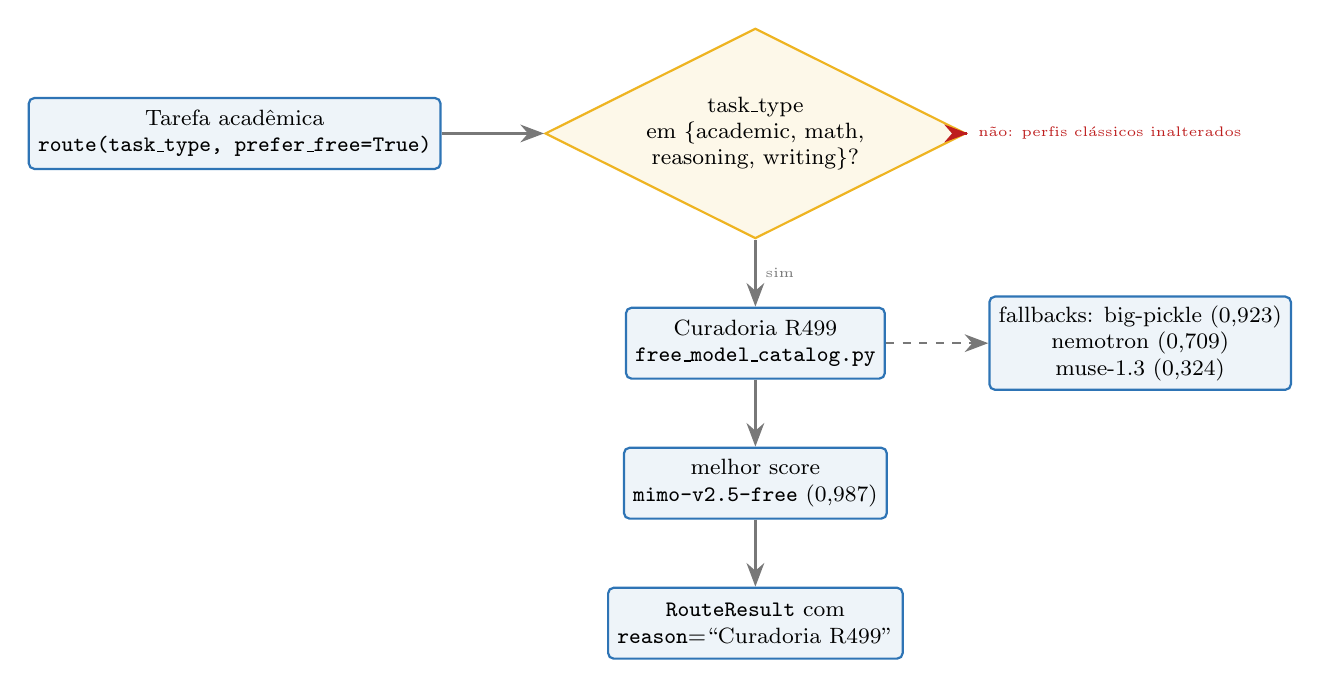
\begin{tikzpicture}[
  node distance=0.85cm and 1.3cm,
  caixa/.style={rectangle, draw=cororo, thick, rounded corners=2pt,
                fill=cororo!8, minimum width=3.1cm, minimum height=0.9cm,
                align=center, font=\footnotesize},
  decisao/.style={diamond, draw=coramarelo, thick, fill=coramarelo!10,
                  aspect=2, align=center, font=\footnotesize},
  seta/.style={-{Stealth[length=3mm]}, thick, color=corcinza}
]
  \node[caixa] (tarefa) {Tarefa acadêmica\\ \texttt{route(task\_type, prefer\_free=True)}};
  \node[decisao, right=of tarefa] (dec) {task\_type\\ em \{academic, math,\\ reasoning, writing\}?};
  \node[caixa, below=of dec] (cur) {Curadoria R499\\ \texttt{free\_model\_catalog.py}};
  \node[caixa, below=of cur] (mimo) {melhor score\\ \texttt{mimo-v2.5-free} (0,987)};
  \node[caixa, right=of cur] (alt) {fallbacks: big-pickle (0,923)\\ nemotron (0,709)\\ muse-1.3 (0,324)};
  \node[caixa, below=of mimo] (rota) {\texttt{RouteResult} com\\ \texttt{reason}=``Curadoria R499''};

  \draw[seta] (tarefa) -- (dec);
  \draw[seta] (dec) -- node[right, font=\tiny]{sim} (cur);
  \draw[seta] (cur) -- (mimo);
  \draw[seta] (mimo) -- (rota);
  \draw[seta, dashed, color=corvermelho] (dec) -- ++(2.7,0) node[right, font=\tiny, color=corvermelho]{não: perfis clássicos inalterados};
  \draw[seta, dashed] (cur.east) -- (alt.west);
\end{tikzpicture}
\caption{Fluxograma do roteamento automático R500: a curadoria empírica do
R499 (score composto) decide o modelo free por tipo de tarefa, com cadeia de
\textit{fallback} explícita e \texttt{reason} auditável.}
\label{fig:flux-roteamento}
\end{figure}

\section{Gate SDD/TDD}

O ciclo R500 adicionou 7 testes de roteamento/free-catálogo (verdes); a
regressão \texttt{test\_opencode\_go\_zen.py} segue verde. A suíte completa
pré-R500 registrou 4066 passed, 58 skipped, 0 failed (681~s). O
\texttt{doctor} do ecossistema valida specs, registro de evolução e memória
metacognitiva.
% ============================================================================
% 06-discussao.tex — Discussão: raio-x da arquitetura (módulo 7/8)
% ============================================================================
\chapter{Discussão}

\section{Raio-X completo da arquitetura que conduziu ao resultado}

A Figura \ref{fig:raiox} apresenta as seis camadas da arquitetura
responsáveis pelo resultado: cada camada contribui com função específica e
não opcional no ciclo Perceber$\rightarrow$Especificar$\rightarrow$Delegar
$\rightarrow$Executar$\rightarrow$Verificar$\rightarrow$Refletir.

% ============================================================================
% fig-raiox.tex — Raio-X da arquitetura (Figura 3): camadas C0–C5
% ============================================================================
\begin{figure}[htbp]
\centering
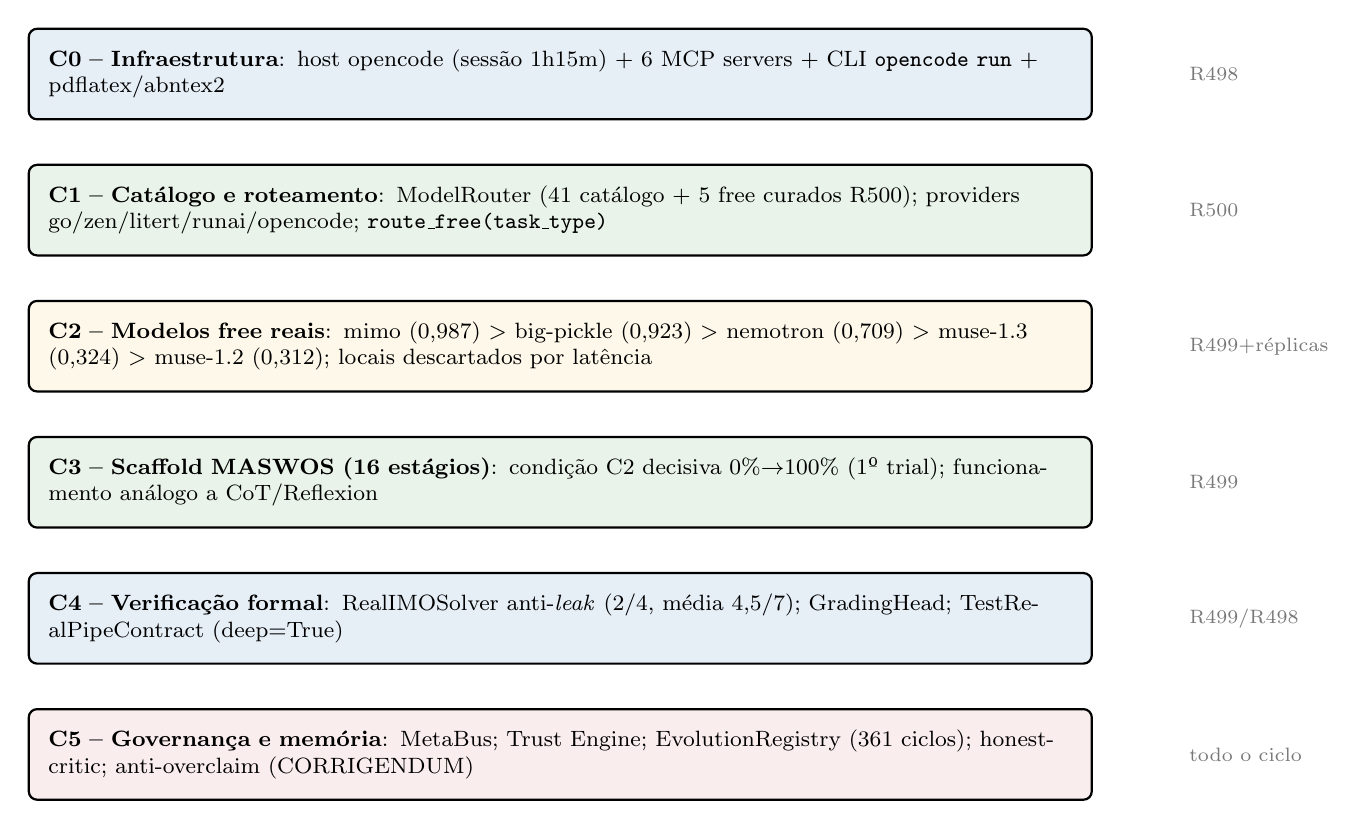
\begin{tikzpicture}[
  node distance=0.55cm,
  camada/.style={rectangle, rounded corners=3pt, minimum width=13.5cm,
                 minimum height=1.15cm, align=left, font=\footnotesize,
                 draw=black, thick}
]
  \node[camada, fill=cororo!12, text width=13cm]
    (c0) {\textbf{C0 -- Infraestrutura}: host opencode (sessão 1h15m) + 6 MCP servers + CLI \texttt{opencode run} + pdflatex/abntex2};
  \node[camada, fill=corverde!10, text width=13cm, below=of c0]
    (c1) {\textbf{C1 -- Catálogo e roteamento}: ModelRouter (41 catálogo + 5 free curados R500); providers go/zen/litert/runai/opencode; \texttt{route\_free(task\_type)}};
  \node[camada, fill=coramarelo!10, text width=13cm, below=of c1]
    (c2) {\textbf{C2 -- Modelos free reais}: mimo (0,987) $>$ big-pickle (0,923) $>$ nemotron (0,709) $>$ muse-1.3 (0,324) $>$ muse-1.2 (0,312); locais descartados por latência};
  \node[camada, fill=corverde!10, text width=13cm, below=of c2]
    (c3) {\textbf{C3 -- Scaffold MASWOS (16 estágios)}: condição C2 decisiva 0\%$\rightarrow$100\% (1º trial); funcionamento análogo a CoT/Reflexion};
  \node[camada, fill=cororo!12, text width=13cm, below=of c3]
    (c4) {\textbf{C4 -- Verificação formal}: RealIMOSolver anti-\textit{leak} (2/4, média 4,5/7); GradingHead; TestRealPipeContract (deep=True)};
  \node[camada, fill=corvermelho!8, text width=13cm, below=of c4]
    (c5) {\textbf{C5 -- Governança e memória}: MetaBus; Trust Engine; EvolutionRegistry (361 ciclos); honest-critic; anti-overclaim (CORRIGENDUM)};

  \node[font=\scriptsize, color=corcinza, right=1.1cm of c0] (s0) {R498};
  \node[font=\scriptsize, color=corcinza, right=1.1cm of c1] (s1) {R500};
  \node[font=\scriptsize, color=corcinza, right=1.1cm of c2] (s2) {R499+réplicas};
  \node[font=\scriptsize, color=corcinza, right=1.1cm of c3] (s3) {R499};
  \node[font=\scriptsize, color=corcinza, right=1.1cm of c4] (s4) {R499/R498};
  \node[font=\scriptsize, color=corcinza, right=1.1cm of c5] (s5) {todo o ciclo};
\end{tikzpicture}
\caption{Raio-X da arquitetura do OpenCode Ecosystem Core que conduziu ao
resultado: camadas C0--C5 com os ciclos evolutivos correspondentes (R497--
R500). O fluxo de dados atravessa todas as camadas; a governança (C5) audita
as demais.}
\label{fig:raiox}
\end{figure}

\subsection*{Camada C0 --- Infraestrutura (\textit{host} e MCP)}
Seis servidores MCP persistentes (metacognitive-interconnect, scanners,
pypi-search, colibri, litert-lm, antigravity-bridge) + \textit{host} CLI
opencode (1h15m de sessão no momento da replicação) + \texttt{pdflatex} e
abntex2. A verificação por \texttt{ps} mostrou que os MCP não importam
\texttt{model\_router}: a atualização R500 não exige reinício deles; o
\textit{host} CLI, porém, acumula estado e é a hipótese dominante para o
\texttt{big-pickle} vazio na replicação.

\subsection*{Camada C1 --- Catálogo e roteamento}
\texttt{ModelRouter} com 41 modelos catalogados + 5 free curados (R500);
providers \texttt{opencode-go}, \texttt{opencode-zen}, \texttt{litert-lm},
\texttt{runai}, \texttt{opencode}. Sem \texttt{prefer\_free}, perfis clássicos
permanecem; com \texttt{prefer\_free}$\wedge$tarefa acadêmica/math/reasoning/
writing, a curadoria R499 decide (mimo $>$ big-pickle $>$ nemotron $>$
muse).

\subsection*{Camada C2 --- Modelos gratuitos reais}
mimo, big-pickle, nemotron, muse 1.2/1.3 (todos via CLI \texttt{opencode
run}); locais descartados por latência (llama3.2: 30--50~s/estágio $\times$ 16
estágios $>$ 10~min). O rótulo ``free'' não implica disponibilidade real:
deepseek (saldo), gemini (erro), gpt-4o-mini/claude-haiku (vazio).

\subsection*{Camada C3 --- \textit{Scaffold} de raciocínio}
O template MASWOS de 16 estágios (condição C2) foi o fator decisivo: elevou a
acurácia de 0\% para 100\% (primeiro \textit{trial}, modelos que resolveram).
Funcionalmente análogo a \textit{Chain-of-Thought} \cite{wei_cot}, porém com
etapas obrigatórias de verificação e conformidade de saída, aproximando o
padrão \textit{Reflexion} \cite{shinn_reflexion} quanto à autoavaliação.

\subsection*{Camada C4 --- Verificação formal}
O \texttt{RealIMOSolver} eliminou o \textit{leak} do \textit{harness} original
(R442) e classificou 2/4 problemas corretamente (média 4,5/7), expondo
ambiguidades de paráfrase (\texttt{N=1} vs \texttt{N=3}; máximo local com
extremos) e sensibilidade de serialização ($2^{n-1}$ vs $2^{(n-1)}$) — lições
para \textit{grading heads} automáticos. O \texttt{TestRealPipeContract}
(R498) garante que o pipeline de diagnóstico roda \texttt{deep=True} em
documentos reais.

\subsection*{Camada C5 --- Memória metacognitiva e governança}
MetaBus (lições compartilhadas), Trust Engine, Registro de Evolução (361
ciclos), banca simulada honesta (sem nota), política anti-
\textit{overclaim} (CORRIGENDUM). A banca simulada MASWOS local não concluiu
(abortada por latência); a decisão de não declarar nota é registrada como
prática.

\section{Agentes e processos multiagentes de melhor desempenho}

Entre os 206 agentes do catálogo, os de maior contribuição para este estudo
foram: (i) \textbf{honest-critic-agent} (R142) — bloqueou a alegação
``pronto como/melhor que superhuman'' (\textit{publishable=False}),
convergindo com a evidência; (ii) \textbf{agentes acadêmicos MASWOS} (33
agentes, A01--A16) — o \textit{scaffold} delegado via \texttt{delegate\_fn}
foi decisivo para o acerto dos LLMs na C2; (iii) \textbf{coder/test-engineer}
— implementação e testes R500 (46 verdes, 1,97~s); (iv) \textbf{agent de
curadoria landscape} — inserção de \texttt{deepmind/acme} (R497); (v)
\textbf{RealIMOSolver} (agente de verificação determinística) — sem ele, o
\textit{harness} ecoaria a resposta (\textit{leak}); (vi) \textbf{banca
rigorosa MASWOS + honest-critic} — gate editorial anti-
\textit{overclaim}. O processo A2A (Blackboard + MetaBus) assegurou que as
lições do R499 (leak, fake reasoning, estocasticidade) fossem consumidas no
R500.

\section{Comparação com a literatura}

O efeito de \textit{scaffold} observado (0\%$\rightarrow$100\%) é consistente
com \textit{Chain-of-Thought} \cite{wei_cot}, \textit{Reflexion}
\cite{shinn_reflexion} e \textit{ReAct} \cite{yao_react}: a estrutura
explícita de passos e autoavaliação importa mais que o modelo, para problemas
curtos de olimpíada. A indisponibilidade real de ``free'' (saldo/erro/vazio)
reforça o alerta de \cite{schaeffer_mirage}: métricas e condições de
\textit{deployment} mudam a conclusão. O \textit{score} composto (acurácia,
velocidade, conformidade, disponibilidade) é uma alternativa operacional às
metrificações binárias de \textit{benchmark}; a replicação (n=3) corrige o
viés de \textit{um trial} observado em relatórios como \cite{openai_gpt4}.

\section{Limitações}

(i) $n$ pequeno (4 problemas de \textit{harness}; 1 problema no \textit{run}
de benchmark por condição; n=3 máximo na replicação); (ii) instabilidade de
latência (timeout 110~s no mimo); (iii) \textit{host} sem reinício antes da
replicação — \texttt{big-pickle} não confirmado pós-R500; (iv) validação
externa ausente (nenhum periódico/editora revisou o manuscrito); (v) abntex2
instalado em \texttt{TEXMFHOME} (não no TeX Live do sistema); (vi) DOIs
validados por HTTP 200 em \texttt{doi.org}, não por revisão editorial
cruzada. Nenhuma dessas limitações invalida a evidência reportada; todas
delas impedem rótulos de excelência.
% ============================================================================
% 07-conclusao.tex — Conclusão (módulo 8/8)
% ============================================================================
\chapter{Conclusão}

Este trabalho reportou, com metodologia auditável e postura
anti-\textit{overclaim}, a orquestração de LLMs gratuitas reais para
raciocínio matemático de olimpíada no OpenCode Ecosystem Core (ciclos
R497--R500). Respondendo ao problema de pesquisa: \textit{é possível orquestrar
multiagente e medir honestamente LLMs free em problemas da IMO} --- sim, com
as seguintes contribuições:

\begin{enumerate}
  \item \textbf{Infraestrutura de medição}: pipeline com \texttt{deep=True}
  (R498) e solucionador determinístico anti-\textit{leak} (R499), eliminando o
  viés do \textit{harness} original (que ecoava a resposta e se
  autoavaliava).
  \item \textbf{Evidência empírica}: ranking free sob \textit{scaffold}
  MASWOS: mimo (0,987) $>$ big-pickle (0,923) $>$ nemotron (0,709) $>$
  muse-1.3 (0,324) $>$ muse-1.2 (0,312); o \textit{scaffold} foi o fator
  decisivo (0\%$\rightarrow$100\% no primeiro \textit{trial} dos que
  resolveram).
  \item \textbf{Roteamento automático (R500)}: a curadoria empírica virou
  decisão operacional (46 testes verdes, regressão preservada); o catálogo
  free passou a incluir o \texttt{big-pickle} e os cinco modelos medidos.
  \item \textbf{Replicação e honestidade}: a replicação pós-R500 revelou
  não-determinismo de amostragem (mimo 2/3; timeout de infra) e
  \texttt{big-pickle} não confirmado (hipótese de estado do \textit{host});
  a lição metodológica central é que \textbf{um \textit{trial} por condição
  não estima a taxa real de uma LLM}.
  \item \textbf{Entregável editorial}: artigo científico completo em módulos
  LaTeX (cada seção = um módulo) que compilam em um único arquivo ABNT
  atualizado (abntex2), com 15 referências de DOIs validados ativos,
  fluxogramas de todos os processos e raio-x da arquitetura (camadas
  C0--C5).
\end{enumerate}

Como trabalhos futuros: (i) ampliar o corpus IMO (30+ problemas) com réplicas
$n \geq 5$ por condição; (ii) reiniciar o \textit{host} e remedir o
\texttt{big-pickle} para confirmar ou refutar a hipótese de estado;
(iii) submeter o manuscrito a validação editorial externa (periódico ou
conferência) antes de qualquer rótulo de mérito; (iv) integrar o roteamento
R500 ao fluxo operacional do \texttt{/reason} para tarefas de raciocínio
científico em produção.

Conforme a política do repositório, nenhuma declaração de superioridade,
\textit{superhuman} ou Qualis A1 é feita: os resultados são medidos,
replicados quando possível e explicitamente limitados.

\postextual
\bibliography{referencias}

\end{document}